\documentclass{eeict}
\inputencoding{utf8}
\usepackage[bf]{caption2}
\usepackage{amssymb}
\usepackage{amsmath}
\usepackage{dsfont}


\newtheorem{example}{Example}[section]
%--------------------------------------------------------------------------------

\title{Decision procedure for WS$k$S}
\author{Tomáš Fiedor}
\programme{Master Degree Programme 2, FIT BUT}
\emails{xfiedo01@stud.fit.vutbr.cz}

\supervisor{Ondřej Lengál}
\emailv{ilengal@fit.vutbr.cz}

\abstract{Various types of logics are often used as means for a formal
specification of systems. The weak monadic second-order logic with $k$
successors (WS$k$S) is one of these logics with quite high expressivity, yet
still is decidable. Although the complexity of checking satisfiability of
WS$k$S formula is not even in ELEMENTARY class, there are some approaches to
this problem that perform well in practice. With a recently developed
techniques for efficient manipulation of non-deterministic tree automata we
want to design and implement a decision procedure for WS$k$S based on
non-deterministic tree automata.}
\keywords{formal verification, tree automata, WS$k$S, decision procedures}

\begin{document}

\maketitle

%-------------------------------------------------------------------------------
\selectlanguage{english}
\section{Introduction}

In formal verification logics are often used for specification of verified
systems in very natural and intuitive way due to their great expressiveness.
However with great expressiveness comes great complexity, when some stronger
logics are not decidable at all.

The WS$k$S \cite{wsks} stands for weak monadic second-order logic of $k$
successors, which means that it allows to quantify over a finite set variables where every element
from the universe of discourse has $k$ successors. This way various $k$-ary tree
structures, e.g. heaps or binary trees, and linear structures, e.g. linked
lists, can be expressed.

There has been several attempts to implement a decision procedure for WS$k$S
using deterministic automata \cite{mona}. However with recent
developments in non-deterministic automata algorithms there is an opened way
for usage of non-deterministic automata.

\section{WS$k$S syntax}

A WS$k$S \emph{term} is either an empty constant $\epsilon$, a first-order
variable symbol written in lower-case letters (e.g. $x$, $y$, \ldots) or an
unary symbol from $\{1,\ldots,n\}$ written in postfix notation. For example
$x1123$ or $\epsilon 2111$ are terms. The \emph{atomic formulae}, for terms $s$
and $t$, is either the equality $s = t$, inequality $s \leq t$ or $s \geq t$, or the membership constraint $t \in
X$, for some second-order variable $X$. The WS$k$S \emph{formula} is then built
out of these atomic formulae using the classical logical connectives $\wedge, \vee, \neg, \Leftarrow, \Leftrightarrow$
and quantifiers $\exists x, \forall x$ and $\exists X, \forall X$ for
quantification over first-order variables and second-order variables
respectively.

\begin{example} Following WS$k$S formula denotes that there exists a singleton
set which is not subset of set $X$.
\begin{equation}
 \varphi = \exists P: Sing(P) \wedge\neg P \subseteq X \label{varphi}
\end{equation}
\end{example}

\section{Deciding WS$k$S}

Deciding logic means classifying whether given formula is \emph{valid},
\emph{invalid}, but \emph{satisfiable} (additionally yielding some assignments)
or \emph{unsatisfiable}. Decision procedure for WS$k$S makes use of a close link
of formulae and automata, i.e. given formula is transformed to correspondent automata and its language is
further examined as shown on Figure \ref{example}

\subsection{Deciding WS$k$S using deterministic automata}

One of the tools for deciding WS$k$S, MONA \cite{mona}, constructs automaton
$\mathcal{A}_\varphi$ for given formula $\varphi$	by structural induction on
formula.
As a base each atomic subformulae is transformed to a correspondent automaton.
Then as an induction step, by considering only logical connectives from
restricted syntax \cite{tata}, we construct for $\vee$, $\neg$ and $\exists$,
union of automata, complement of automaton and $i$-th projection of automaton respectively.

\begin{figure}
 \begin{center}
  \scalebox{0.7}{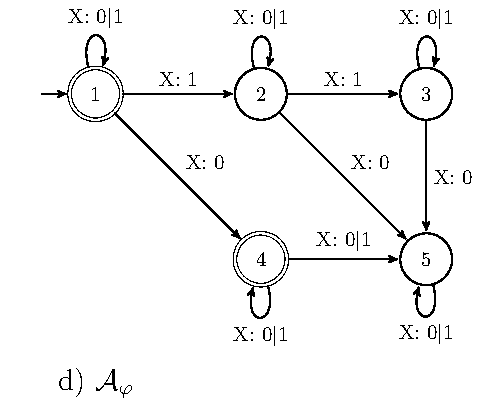
\includegraphics{formula-automaton.pdf}}
 \end{center}
 \caption{Automaton corresponding to example formula $\varphi = \exists P:
 Sing(P) \wedge\neg P \subseteq X$}\label{example}
\end{figure}

\subsection{Deciding WS$k$S using non-deterministic automata}

Despite having good computational results in practice, every time a non-determinism is introduced the automaton
is determinised and thus information about the original states is forgotten.

So such an approach has issues with extensive usage of automaton complementation
and since currently there is no known tree automaton complementation technique
better than bottom-up determinization of automaton with complementation of the
final states, heavy optimizations and heuristics had to be used in MONA for
achieving good results.

We propose that it is not necessary to construct the automaton representing all
models of $\varphi$. Instead the automaton and the search for an accepting or
non-accepting state can be done \emph{on-the-fly} and exploit recent development
in algorithms using non-deterministic automata. 

Given a WS$k$S formula $\varphi$ we transform it to the formula in 
\emph{existentially-quantified prenex normal form} $\psi =
\exists\mathcal{X}_{m+1}\neg\exists\mathcal{X}_m\ldots\neg\exists\mathcal{X}_2\neg\exists\mathcal{X}_1.\pi(\mathds{X})$,
where $\mathcal{X}_i$ denotes set of second order variables.
We then create a hierarchical family of WS$k$S formulae $\varphi =
\{\varphi_0,\ldots,\varphi_m\}$ where $\varphi_0 = \pi$ and for all $0 \leq i \leq
m-1$ it holds that $\varphi_{i+1} = \neg\exists\mathcal{X}_{i+1}\varphi_i$. 

Further using the operations of complementation $\gamma$ and projection
$\omega_{\mathcal{X}}$ over set of variables $\mathcal{X}$ we define the family
of automata $\mathds{A} = \{\mathcal{A}_0,\ldots,\mathcal{A}_m\}$ as following:
\begin{eqnarray}
 \mathcal{A}_0 & = & \mathcal{A}_\pi\\
 \mathcal{A}_{i+1} & = & \gamma(\omega_{\mathcal{X}_{i+1}} (\mathcal{A}_i)), 0 <
 i < m - 1
\end{eqnarray}

Language of these automata are further tested for universality. The classical
naive approach performs a determinization using a subset construction to obtain
a deterministic automaton, which is further complemented and finally being
checked if there is no reachable state in this automaton.

Proposed algorithm \cite{anti} runs the subset construction on-the-fly and
checks if any rejecting macro-state, i.e. a subset of states $Q$ of automaton,
is reachable based on worklist algorithm. Macro-states from worklist are expanded and
their successors $S$ are moved to process, unless there exists some other
macro-state $R$ already expanded such that for all states in $S$ there exists
some state in $R$ in $\preceq$ relation, where $\preceq \subseteq Q \times Q$ is
some relation implicating inclusion over languages accepted from states.

Let us take automaton for our example formula \ref{varphi} depicted on Figure
\ref{example}. By classical approach 7 states are generated as shown
on Figure \ref{compare}. If we use the antichain based approach then
macro-states $\{1, 4\}$ and $\{1, 2\}$ are simulated by initial state $\{1\}$,
so we don't expand these states any further and the construction of automaton
ends.
Since we did not reach any accepting state, we can conclude that language is not
universal and formula is thus not valid.

\begin{figure}
 \begin{center}
  \scalebox{0.5}{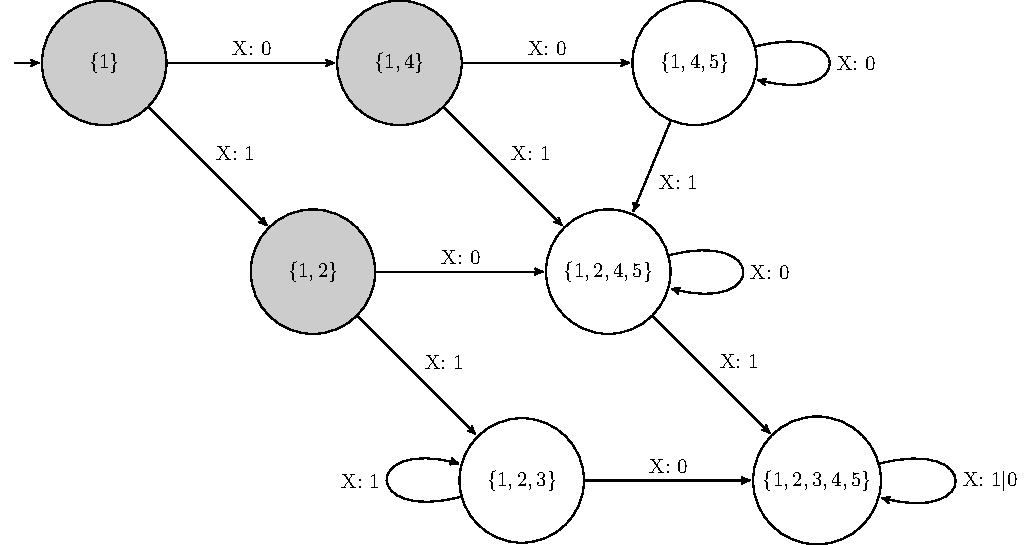
\includegraphics{antichain-meets-projection.pdf}}
 \end{center}
 \caption{Comparison of antichain based (grey nodes) and classical approach to
 universality checking of formula $\varphi = \exists P: Sing(P) \wedge\neg P
 \subseteq X$}\label{compare}
\end{figure}

\section{Conclusion}

We proposed a new decision procedure of WS$k$S logic that uses non-deterministic
automata instead of deterministic ones used in classical approach, f.e. in tool
MONA \cite{mona}. This different approach makes use of a recent developments in
fields of non-deterministic automata algorithms like universality checking or
language inclusion, allowing us to search for a rejecting or accepting states
on-the-fly without constructing automaton corresponding to the given formula at
all, possible yielding better computational results for some types of formulae.

%------------
% Citace
%------------
\begin{thebibliography}{9}
%  \bibitem{anti}Abdulla, Parosh Aziz, Hol\'{i}k, Luk\'{a}\v{s}, Chen, Yu-Fang,
%  Mayr, Richard, Vojnar, Tom\'{a}\v{s}.: When simulation meets antichains (on
%  checking language inclusion on nondeterministic finite (tree) automata). In
%  \emph{Tools and Algorithms for Construction and Analysis of Systems}, LNCS
%  6015, pages 158-174, Springer Verlag, 2010.
\bibitem{anti}Hol\'{i}k, Luk\'{a}\v{s}, et. al.: When simulation meets
antichains (on checking language inclusion on nondeterministic finite (tree) automata). In
  \emph{Tools and Algorithms for Construction and Analysis of Systems}, LNCS
  6015, pages 158-174, Springer Verlag, 2010.
  \bibitem{mona}MONA:
  Web pages of MONA.
  [online] Available on:
  http://www.brics.dk/mona/, Last Visited January 2014.
  \bibitem{tata}Comon, H. et al.: Tree automata techniques and applications.
  2007, release October, 12th 2007.
  \bibitem{wsks}Büchi, J. R.: Weak second-order arithmetic and finite automata.
  \emph{Mathematical Logic Quarterly}, 6(1-6):66-92, 1960.
\end{thebibliography}

\end{document}
